\documentclass[border=10pt]{standalone}
\usepackage[svgnames]{xcolor}
\usepackage{amsmath}
\usepackage{pgfplots}
\pgfplotsset{compat=newest}
\usepackage[sfdefault]{FiraSans}
\usepackage{FiraMono}
\renewcommand*\familydefault{\sfdefault}
\begin{document}
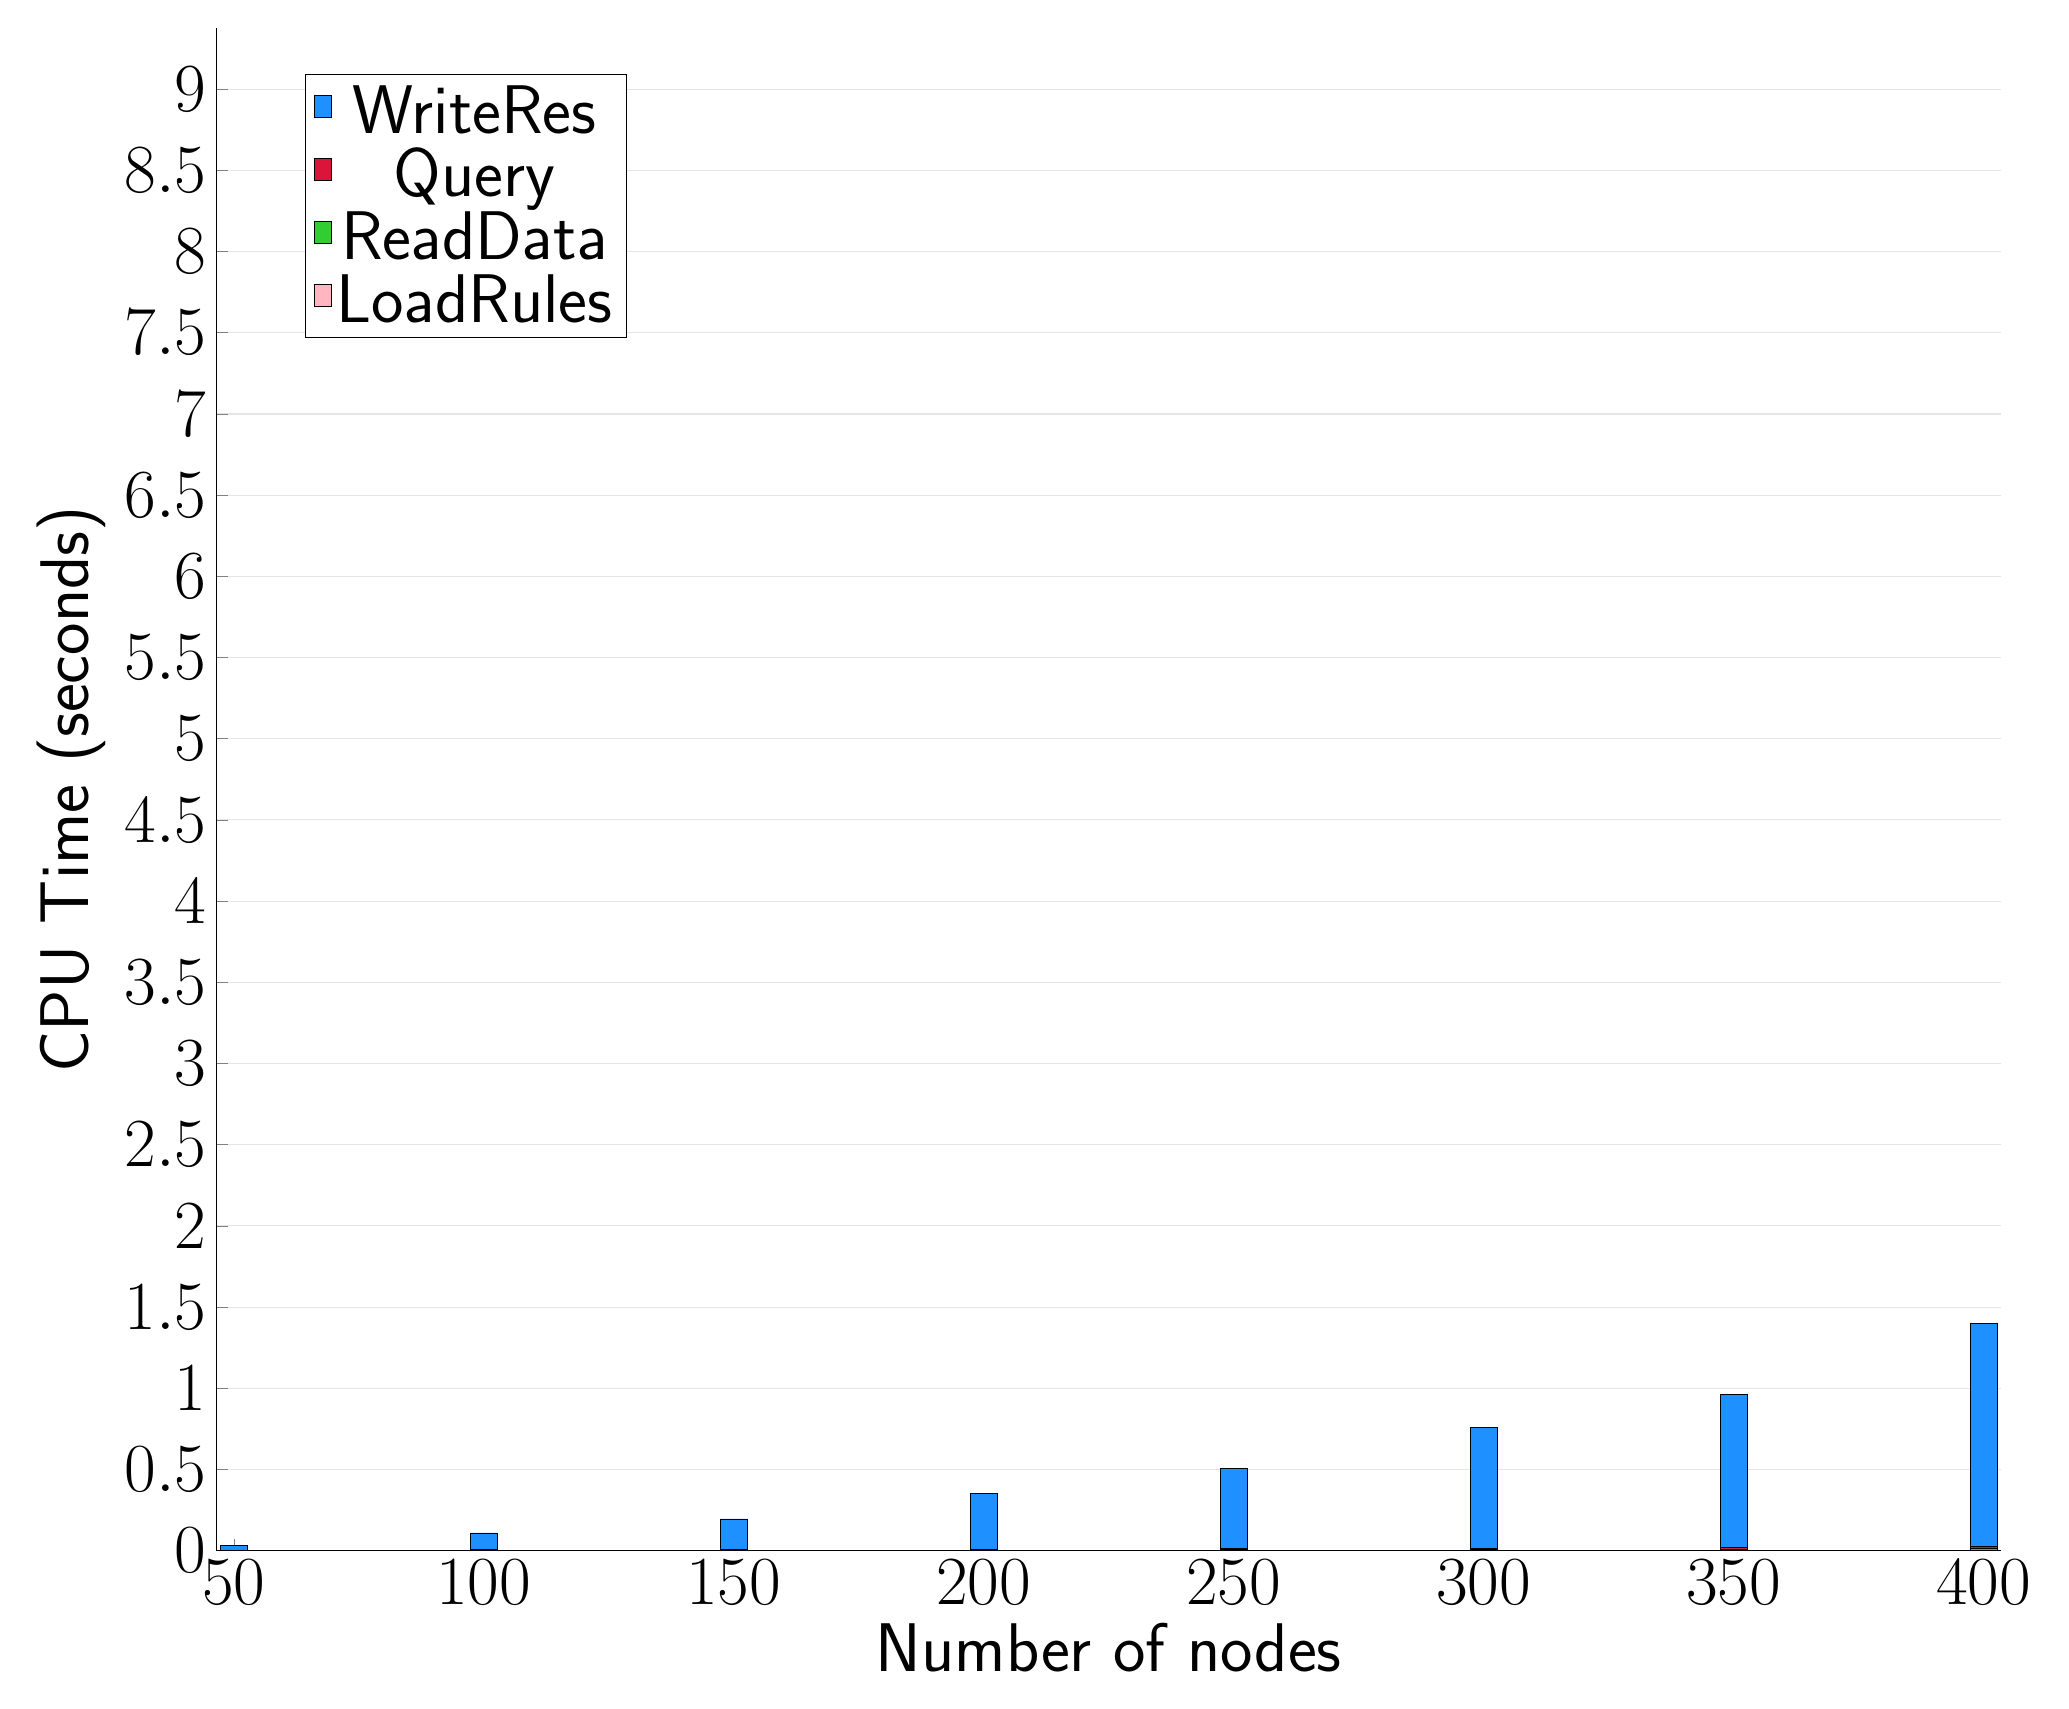
\begin{tikzpicture}
\begin{axis}[
   ybar stacked,
   width=2\textwidth,
   bar width=0.35cm,
   ymajorgrids, tick align=inside,
   major grid style={draw=gray!20},
   xtick=data,
   ymin=0, ymax=9.375487327575684,
   axis x line*=bottom,
   axis y line*=left,
   enlarge x limits=0.01,
   legend style={
       at={(0.23, 0.97)},
       anchor=north east,
       legend columns=1,
       font=\Huge,
   },
   ylabel={CPU Time (seconds)},
   xlabel={Number of nodes},
   label style={font=\Huge},
   tick label style={font=\Huge},
]
\addlegendimage{fill=DodgerBlue, draw=black, line width=0.2pt}
\addlegendentry{WriteRes}
\addlegendimage{fill=Crimson, draw=black, line width=0.2pt}
\addlegendentry{Query}
\addlegendimage{fill=LimeGreen, draw=black, line width=0.2pt}
\addlegendentry{ReadData}
\addlegendimage{fill=LightPink, draw=black, line width=0.2pt}
\addlegendentry{LoadRules}
\addplot +[fill=LightPink, draw=black, line width=0.2pt] coordinates {
(50, 0.0032606666666666665)
(100, 0.0032133333333333337)
(150, 0.002800333333333333)
(200, 0.002263)
(250, 0.002668666666666667)
(300, 0.002526333333333333)
(350, 0.0035923333333333332)
(400, 0.0034436666666666665)
};
\addplot +[fill=LimeGreen, draw=black, line width=0.2pt] coordinates {
(50, 0.0012826666666666663)
(100, 0.0026130000000000003)
(150, 0.0032823333333333333)
(200, 0.004690333333333334)
(250, 0.005468666666666666)
(300, 0.005395333333333333)
(350, 0.0073149999999999995)
(400, 0.00901066666666666)
};
\addplot +[fill=Crimson, draw=black, line width=0.2pt] coordinates {
(50, 0.00015066666666666465)
(100, 0.000766333333333334)
(150, 0.0015393333333333333)
(200, 0.003161666666666667)
(250, 0.004079333333333337)
(300, 0.006049333333333334)
(350, 0.008550666666666666)
(400, 0.013493333333333335)
};
\addplot +[fill=DodgerBlue, draw=black, line width=0.2pt] coordinates {
(50, 0.02644366666666667)
(100, 0.102393)
(150, 0.18811666666666663)
(200, 0.3426403333333334)
(250, 0.4947473333333334)
(300, 0.7448043333333333)
(350, 0.94062)
(400, 1.3726166666666666)
};
\end{axis}
\end{tikzpicture}

\end{document}
